% !TeX program = xelatex
\documentclass{resume}
\ResumeName{Shaojie Tan}

\usepackage{graphicx}
\usepackage{tikz}
\linespread{1.04}\selectfont

\begin{document}

\ResumeContacts{
  \ResumeUrl{mailto:943648187@qq.com}{943648187@qq.com},%
  \ResumeUrl{https://shaojiemike.top}{shaojiemike.top},%
  \ResumeUrl{https://github.com/Kirrito-k423}{github.com/Kirrito-k423}%
}

\begin{tikzpicture}[remember picture,overlay]
  \node[anchor=north east,inner sep=1cm] at (current page.north east)
    {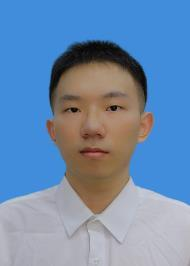
\includegraphics[width=1.85cm]{photo.jpg}};
\end{tikzpicture}

\ResumeTitle

\noindent M.S. in Computer Science from the University of Science and Technology of China, focused on computer architecture, high-performance computing, parallel optimization, and PIM task scheduling, with hands-on experience from microarchitectural analysis to multi-node CPU/GPU optimization.

\section{Education}
\ResumeItem{University of Science and Technology of China}[M.S. in Computer Science][Sep 2021--Jun 2024]
\ResumeItem{University of Science and Technology of China}[B.S. in Computer Science][Sep 2017--Jun 2021]

\section{Research \& Internship}
\ResumeItem{Huawei 2012 Laboratories}[Research Intern · PIM Task Scheduling][Jul 2023]
\begin{itemize}
  \item Built a compile-time performance model and reduced data movement through locality and connectivity clustering.
  \item Selected execution between PIM and CPU using parallelism and memory-port pressure, achieving near-optimal scheduling with static analysis alone.
\end{itemize}

\ResumeItem{USTC × Huawei}[Kunpeng 920 Basic-Block Throughput Modeling][Sep 2021--Nov 2022]
\begin{itemize}
  \item Developed a throughput prediction framework and benchmark suite using instruction throughput, latency, and port-pressure data.
  \item Improved llvm-mca accuracy on AArch64 by modeling the Kunpeng 920 microarchitecture; published at IEEE HPCC 2022.
\end{itemize}

\section{Selected Projects}
\ResumeItem{Multi-GPU Quantum Circuit Simulation with QuEST}[ASC20-21 First Prize][Nov 2020--May 2021]
\begin{itemize}
  \item Enabled direct GPU-memory access with CUDA-aware MPI, overlapped computation and communication, and replaced reductions with cuBLAS.
  \item Scaled from 30 to 34 qubits on 8 NVIDIA A100 GPUs across 4 nodes, saving more than 200 GB versus the CPU system.
\end{itemize}

\ResumeItem{Multi-node CPU Optimization}[IPCC 2022 Third Prize · 5/130+][Jul 2022--Nov 2022]
\begin{itemize}
  \item Combined loop unrolling, manual vectorization, OpenMP, and MPI; optimized data layout, mixed precision, and PSRS-based hotspots.
  \item Reached 10,000× speedup on dual AMD EPYC 7452 nodes and up to 2,800,000× on a single node.
\end{itemize}

\section{Technical Skills}
\begin{itemize}
  \item \textbf{Programming:} C, C++, Python, Shell. \textbf{Parallel computing:} MPI, OpenMP, CUDA, cuBLAS.
  \item \textbf{Architecture:} Intel/ARM ISA, AArch64, CPU microarchitecture, PIM, performance modeling. \textbf{Analysis:} assembly, vectorization, cache and bandwidth optimization, llvm-mca.
\end{itemize}

\section{Awards \& Publication}
\begin{itemize}
  \item First Prize, ASC20-21 Student Supercomputer Challenge Finals; First Prize, ISC21 Student Cluster Competition Finals.
  \item Qingcai Jiang, \textbf{Shaojie Tan}, Zhenwei Cao, et al. ``Quantifying Throughput of Basic Blocks on ARM Microarchitectures by Static Code Analyzers: A Case Study on Kunpeng 920.'' \textbf{IEEE HPCC 2022}.
\end{itemize}

\end{document}
